\documentclass[]{article}
\usepackage[ngerman]{babel}
\usepackage{natbib}
\usepackage{graphicx}
\usepackage{qtree}
\usepackage[utf8]{inputenc}

%opening
\title{Abschlussbericht Semantic Argument Classification}
\author{Julian Baumann, Kevin Decker, Maximilian Müller-Eberstein}


\begin{document}

\maketitle

\section{Einleitung}
Unter Semantic Argument Classification versteht man, einem Satz seine semantische Rollen wie zum Beispiel Agens, Patiens etc. zuzuweisen. Vereinfacht gesagt versucht man zu klären, \glqq wer wem was antut\grqq. Beispielsweise würde der Satz \glqq It operates stores mostly in Iowa and Nebraska\grqq folgendermaßen annotiert werden: $ [_{\textbf{Arg0}} It][_{\textbf{Pred}} operates][_{\textbf{Arg1}} stores][_{\textbf{ArgLoc}} mostly\ in\ Iowa\\ and\ Nebraska] $. Sie gehört zum grundlegenden Pre-Processing für verschiedene Natural Language Processing-Anwendungen wie zum Beispiel Machine Translation und ist aus diesem Grunde auch ein wichtiger Aspekt der Forschung. \\
Angelehnt an die Veröffentlichung von \cite{Pradhan05supportvector} versuchten wir im Verlauf unseres Projekts diese Aufgabe automatisch und überwacht durch Machine Learning-Ansätze umzusetzen. 

\section{Grundlagen}
\subsection{Daten und Tools}
Als Grundlage für unsere Experimente wurden verschiedene Datensätze und Tools verwendet. Wichtigste Ressourcen waren dabei PropBank und Penn TreeBank. PropBank \cite{Palmer:2005:PBA:1122624.1122628} oder auch Proposition Bank ist ein Annotations-Schema, nach welchem für jedes  Verb annotiert wird, welche semantische Rollen es besetzt. \\ Dies ist in Form von sogenannten Frames organisiert, die kodieren, welche Argumente überhaupt gefordert werden können. Im Gegensatz zu FrameNet, welches das gleiche versucht, ist PropBank jedoch nicht ganz so spezifisch sondern versucht durch algemeinere Kategorien für möglichst viele Parser verwendbar zu sein.\\ 

\begin{table}
	\centering
	\begin{tabular}{|c|l|}
	\hline 
	ARG0 & proto-agent \\ 
	\hline 
	ARG1 & proto-patient \\ 
	\hline 
	ARG2 & instrument, benefactive, attribute \\ 
	\hline 
	ARG3 & starting point, benefactive, attribute \\ 
	\hline 
	ARG4 & ending point \\ 
	\hline 
	ARGM & modifier \\ 
	\hline 
	\end{tabular}
	\caption{Argumente der PropBank}
	\end{table}
	Die Penn TreeBank \cite{Marcus93buildinga} ist ein syntaktisch annotierter Subkorpus des Wall Street Journals(WSJ) bestehend aus etwa einer Millionen Tokens. Davon sind etwa 112.917 Prädikat-Argument Strukuren nach dem PropBank-Schema annotiert. 
	\\
	Die oben genannten Korpora bilden die Grundlage für die im Folgenden näher erklärten Experimente.
	Zur Extraktion der Features wurde die Programmiersprache Python in der Version 3.4 zusammen mit dem Natural Language Toolkit \(Version 3.0\) verwendet. Die eigentliche Anwendung der Machine-Learning Algorithmen wurde in Weka \cite{Hall+FHPRW:2009} realisiert.
	\\
	Zur Klassifikation sollten drei verschieden Algorithmen verwendet werden:
	Der Naïve Bayes und der J48-Algorithmus, sowie eine Support
	Vector Machine. Letztere wurde ausgewählt, um den Experimentausgang mit den Ergebnissen von \cite{Pradhan05supportvector} zu vergleichen, die ebenfalls eine Support Vector Machine verwenden.
	
	
	



%Datenvorstellung, Tools, Algorithmen
%Vergleichsgrundlagen
\section{Umsetzung} 

%umsetzung
\section{Features}
\subsection{einzelne Features}
Für das Experiment wurden 5 Features extrahiert und ihr Einfluss auf die Ergebnisse getestet.\\
Das erste Feature, \textbf{Predicate}, ist einfach die lemmatisierte Form des Prädikats. In unserem Datenset trat dieses Feature in 3966 verschiedenen Werten auf.\\
Zweites Feature, \textbf{Path}, beschreibt den Weg, der in einem Syntaxbaum durchlaufen werden muss, um von einem Argument zum Prädikat der Instanz zu gelangen. Dies wird durch $\uparrow$ und $\downarrow$ gekennzeichnet.

\begin{center}
\Tree [.S [\qroof{The lawyers\\ \textbf{ARG0}}.NP  ] [.VP [.VBD {went\\ \textbf{Predicate}} ] [.PP {to\\ \textbf{Null}} ] [.NP {work\\ \textbf{ARG4}} ] ] ]
\end{center}

Im Satz \glqq The lawyers went to work\grqq\ würde dieses Feature beispielsweise den Wert NP $\uparrow$ S $\downarrow$ VP $\downarrow$ VBD annehmen. Dieses Feature hat sehr viele verschiedene Ausprägungen (41737 distinct values), die durch verschiedene Satzstrukuren verursacht werden.\\ In der Evaluation betrachten wir ebenfalls Vor- und Nachteile der Vereinfachung dieses Features in der Form von bsp. Duplikatbeseitigung (... $\uparrow$ S $\downarrow$ VP $\downarrow$ VP $\downarrow$ ... $\Rightarrow$ ... $\uparrow$ S $\downarrow$ VP $\downarrow$ ... ) oder Pruning (NP $\uparrow$ S $\downarrow$ VP $\downarrow$ ... $\Rightarrow$ NP $\uparrow$). Im Feature \textbf{Phrase Type} ist kodiert, welchem Konstituententypus (also NP, VP, etc.) das gesuchte Argument angehört. In unserem Fall sind dies 65 verschiedene Kategorien, nachdem für unsere Zwecke zu eingrenzende Typen konvertiert wurden (z.B. NP-SUBJ zu NP).\\
Die anderen beiden Features \textbf{Position} und \textbf{Voice} sollten beide intuitiv betrachtet binär sein, durch die unvollständige Annotation in Propbank ist dies im Falle von Voice, also ob das Argument passiv oder aktiv ist, nicht der Fall. Hier gibt es noch einen dritten Wert unknown, wenn für das Prädikat keine Angabe diesbezüglich gemacht wurde. Position hingegen ist ein rein binäres Feature und gibt an, ob das Argument vor oder nach dem Prädikat auftritt. 

\subsection{Featureextraktion}
Das Ziel unserer Featureextraktion bestand darin, die Daten der PropBank und Penn TreeBank mit den oben genannten Features in normalisierter Form zusammenzuführen und in das Weka-kompatible Attribute-Relation File Format (ARFF) zu konvertieren.\\
Instanzen der PropBank liegen in einem Space- und Newline-separierten Textformat vor. Innerhalb einer Instanz verweisen Pointer auf Teilbäume der korrespondierenden Penn TreeBank Sätze, die in einem Klammer-Format annotiert sind.
\begin{center}
	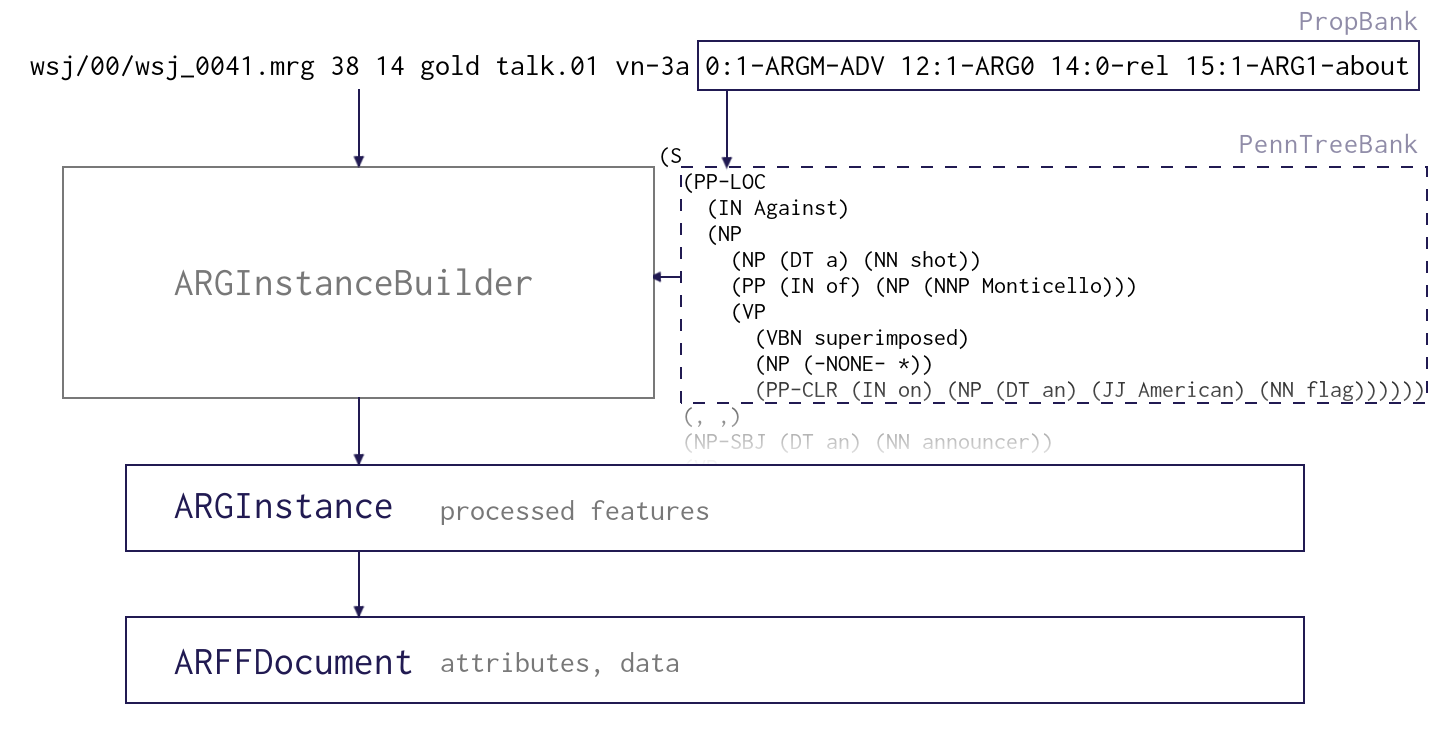
\includegraphics[scale=0.23]{argext_graphic.png}
\end{center}
Mit Hilfe des NLTK, welches die rohen Textdateien beider Korpora in vordefinierte Klassen lädt, erstellen wir ARGInstances, in denen alle Features in normalisierter- und leicht abrufbarer Form vorliegen. Die Helferklasse ARGInstanceBuilder übernimmt die Zusammenführung beider Korpora, die Berechnung des Path-Features mittels Baumtraversierung und Ermittlung des Lowest-Common-Ancestors und ähnliche Extraktionsaufgaben, sowie die finale Normalisierung. Die so generierten ARGInstances werden zuletzt an ein ARFFDocument weitergegeben, welches Trainings-, Development- und Testdaten in ARFF-Dateien schreibt, die direkt mit Weka weiterverarbeitet werden können.

\section{Experimente}
\subsection{Setup}

Wir haben die Daten in 60\% Training 20\% Development und 20\% Test Daten aufgeteilt. 
Als Baselines haben wir die ZeroR Baseline gewählt, da in der Literatur zumeist nur Ergebnisse für die schwierigere Aufgabe Argument Identifikation+Klassifikation zu finden sind. \\
Als Algorithmen benutzen wir Naive Bayes und j48 decision tree mit den Weka Default Einstellungen. \\
Ursprünglich hatten wir auch noch geplant auf einem SVM basierten Algorithmus zu evaluieren. 
Dabei wurden jedoch alle Instanzen der häufigsten Klasse zugeteilt, was an einem unbalancierten Datenset liegen könnte.

\subsection{Feature Selektion auf dem Development set (Naïve Bayes}
\begin{table}[h]
\scalebox{0.9}{
\begin{tabular}{l|lll|l}
                      & Precision      & Recall         & F-Measure      & F-Measure Change \\ \hline
\textit{All Features} & \textit{0.771} & \textit{0.778} & \textit{0.770} & \textit{0}       \\ \hline
-voice               & 0.748          & 0.754          & 0.745          & -0.025           \\
-path                & 0.778          & 0.783          & 0.776          & \textbf{+0.006}  \\
-phraseType          & 0.735          & 0.747          & 0.733          & -0.037           \\
-position            & 0.758          & 0.773          & 0.757          & -0.013           \\
-predicate            & 0.717          & 0.732          & 0.716          & \textbf{-0.054}  
\end{tabular}
}
\end{table}

Auf dem Development Set konnten wir feststellen, dass wir durch das Entfernen des Path Features bessere Ergebnisse erreichen konnten.
Auch weitere Versuche das Path Feature zu verbessern, indem wir aufeinanderfolgende, doppelte Kategorien zusammenfassen und nur den Pfad vom Argument aufwärts benutzen, schlugen fehl. Effektiv verschlechterte das Feature sogar unsere Ergebnisse mit einem Abfall auf 0.738 für den Naïve Bayes und 0.838 für den J48-Algorithmus im F-Measure \\
Deshalb ließen wir dieses Feature, obwohl es im Originalpaper \citep{Pradhan05supportvector} mit einbezogen wurde, aus unserer Evaluierung auf dem Testset raus, um ein besseres Ergebnis zu erzielen. 



\subsection{Test Set Ergebnisse}
\begin{table}[h]
\begin{tabular}{l|lll}
                  & Precision      & Recall         & F-Measure      \\ \hline
\textit{Baseline} & \textit{0.132} & \textit{0.364} & \textit{0.194} \\ \hline
Naïve Bayes       & 0.777          & 0.781          & 0.774          \\
j48 Tree          & 0.847      	   & 0.849            & 0.846          
\end{tabular}
\end{table}

Die von uns mit Bedacht niedrig gelegte ZeroR Baseline konnten wir, wie zu erwarten war, definitiv schlagen. Von den beiden Algorithmen, die wir nach mehreren Durchläufen für am passendsten erachtet hatten, erwies sich der Decision Tree Algorithmus als deutlich effektiver als der Naïve Bayes Algorithmus.\\
Hierbei wird ARG0 sehr präzise klassifiziert und weitet sich dabei allerdings auch merklich in die Instanzen der ARG1-Klasse aus, was bei der letzteren zu einem leichten Abfall im Recall führt. Bei der Unterscheidung von Proto-Agens und -Patiens besteht also ein geringfügiger Bias zu einer Klassifizierung als Agens. Alle weiteren Klassen zeigen stets die größten Überschneidungen mit ihren semantisch ähnlichsten Nachbarn (ARG3 und ARG2, ARG5 und ARGM etc.), was also bedeutet, dass selbst bei einer Missklassifikation die etwaige Valenz beibehalten wird.\\
Insgesamt zeigt sich also, dass, wie zu erwarten, die häufigsten Argumentklassen am besten trainiert und folglich auch am präzisesten klassifiziert werden und sich insbesondere bei den vom Prädikat weiter entfernten Klassen ARG2-ARGM die semantische Ähnlichkeit stark in der Ähnlichkeit der Feature-Werte widerspiegelt.



\section{Retrospektive}
Über den gesamten Projektverlauf hinweg hoben sich einige Aspekte immer wieder hervor.\\
Die Aufgabe der semantischen Argumentklassifikation erwies sich, wie man an den Inhalten der Penn TreeBank sehen kann, als äußerst divers und sehr wichtig für die tiefere Verarbeitung der natürlichen Sprache. Das Annotationschema der PropBank zeigte, dass es ohne größere Schwierigkeiten auf diese verschiedensten semantischen Kontexte appliziert werden kann ohne an Allgemeinheit zu verlieren und somit sehr gut für diverse Machine Learning Methoden geeignet ist.\\
Die Feature-Extraktion und anschließende -Selektion, bei der im Gegenzug versucht werden musste, den allgemeinen und somit auch teils vagen Argumentklassen der PropBank distinktive Features ohne Overfitting zuzuweisen, stellte sich, wie zu erwarten, als der komplexeste Teil des Projektes heraus. Das Path-Feature zeigt wahrscheinlich am deutlichsten, wie selbst nach einer Anpassung und Reduktion der Feature-Werte die Ergebnisse sich nur minimal oder gar nicht verbessern, obwohl es dem ersten Anschein nach eines der wichtigsten Feature zu sein schien, um insbesondere ähnliche Argumentklassen zu unterscheiden.\\
Zuletzt zeigten sich bei den angewandten maschinellen Lernverfahren sowohl die Stärken und Schwächen bei der Verarbeitung von Datensätzen deren Features zahlreiche Werte annehmen. Die SVM, welche ursprünglich an \cite{Pradhan05supportvector} angelehnt, der wichtigste Algorithmus werden sollte, stellte sich (zumindest in den uns vorliegenden Umsetzungen für Weka) wegen Klassenanzahl und der hohen Anzahl an Feature-Werten als ungeeignet heraus. Eventuell hätte eine Balancierung der Daten gewünschte Ergebnisse erzielt. Dies setzt allerdings eine weitere Vorverarbeitung der Daten voraus, die sich von den anderen Algorithmen differenziert hätte.\\
Die Ergebnisse Naïve Bayes sind hingegen wesentlich vielversprechender und zeigen, dass trotz der Einfachheit des Algorithmus unsere Feature distinktiv genug sind um ein F-Measure von rund 77\% zu erreichen. J48 benötigte zwar auf Grund der höheren Komplexität wesentlich mehr Berechnungsressourcen, stellte sich jedoch als signifikant präziser heraus. Dies lässt vermuten, dass das Zusammenspiel der Features wichtiger ist, als das jeweils einzeln betrachtete reine Maximum.\\
Insgesamt ziehen wir also den Schluss, dass die Umsetzung der automatischen semantische Argumentklassifikation mittels Maschinenlernverfahren mit einem allgemein gehaltenen Annotationsschema und einem Algorithmus, der Feature als von einander abhängig betrachtet, bereits sehr zeigenswerte Ergebnisse erzielt werden können.



\bibliographystyle{abbrv}
\bibliography{Quellen}

\end{document}
